\documentclass{standalone}
\usepackage{tikz, pifont}
\usetikzlibrary{trees, shapes, patterns}

\newcommand{\coula}{0785F2}
\newcommand{\coulb}{F29F05}
\newcommand{\coulc}{F21313}
\newcommand{\could}{6698FF}



\definecolor{part1}{HTML}{\coula}
\definecolor{part2}{HTML}{\coulb}
\definecolor{part3}{HTML}{\coulc}
\definecolor{part4}{HTML}{\could}
\begin{document}

% permuto�dre
 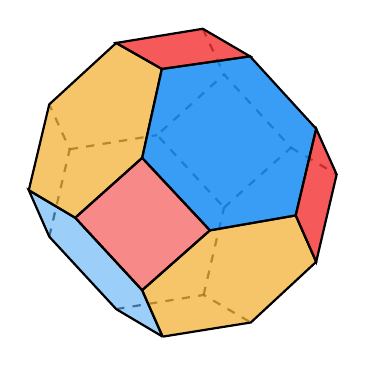
\begin{tikzpicture}[thick]
\coordinate (A1) at (2.63,0.27);
\coordinate (A2) at (3.75,0.45);
\coordinate (A3) at (4.58,1.22);
\coordinate (A4) at (4.84,2.33);
\coordinate (A5) at (4.58,2.91);
\coordinate (A6) at (3.74,3.83);
\coordinate (A7) at (3.14,4.18);
\coordinate (A8) at (2.04,4.00);
\coordinate (A9) at (1.19,3.22);
\coordinate (A10) at (0.93,2.13);
\coordinate (A11) at (1.19,1.54);
\coordinate (A12) at (2.04,0.62);
\coordinate (B1) at (2.37,0.86);
\coordinate (B2) at (3.23,1.62);
\coordinate (B3) at (2.37,2.54);
\coordinate (B4) at (1.52,1.78);
\coordinate (C1) at (3.41,1.91);
\coordinate (C2) at (4.26,2.67);
\coordinate (C3) at (3.41,3.60);
\coordinate (C4) at (2.56,2.83);
\coordinate (D1) at (1.45,2.65);
\coordinate (D2) at (3.15,0.80);
\coordinate (O1) at (4.32,1.81);
\coordinate (O2) at (2.62,3.67);
\begin{scope}[thick,dashed,,opacity=0.6]
\draw (A12) -- (D2)--(A2);
\draw (C1)--(C2)--(C3)--(C4)--(C1);
\draw (A11) -- (D1)--(A9);
\draw (D1)--(C4);
\draw (D2)--(C1);
\draw (C2)--(A4);
\draw (A7)--(C3);
\end{scope}
\draw[fill=part1,fill opacity=0.4] (A1) -- (A12) -- (A11)--(A10)--(B4)--(B1)--(A1);
\draw[fill=part2,fill opacity=0.6] (A1) -- (A2) -- (A3)--(O1)--(B2)--(B1)--(A1);
\draw[fill=part2,fill opacity=0.6] (A10) -- (B4) -- (B3)--(O2)--(A8)--(A9)--(A10);
\draw[fill=part1,fill opacity=0.8] (B3) -- (B2) -- (O1)--(A5)--(A6)--(O2)--(B3);
\draw[fill=part3,fill opacity=0.5] (B1) -- (B2) -- (B3)--(B4)--(B1);
\draw[fill=part3,fill opacity=0.7] (O2) -- (A6) -- (A7)--(A8)--(O2);
\draw[fill=part3,fill opacity=0.7] (O1) -- (A3) -- (A4)--(A5)--(O1);
\end{tikzpicture}
\end{document}
